\section{\texorpdfstring{Jednoduchý program}{Jednoduchy program}}

% =====================================================================================================================
	\begin{frame}
    \frametitle{Zadání}
		
		\begin{enumerate}
			\item Založit proměnnou - 1 byte místo v paměti pojmenované \textbf{moje\_promenna}.
			\item Proměnnou nastavit na předdefinovanou dekadickou hodnotu 150.
			\item Proměnnou postupně odečítat po 1.
			\item Pokud je výsledek proměnné 0, pokračovat bodem 2, jinak pokračovat bodem 3.
		\end{enumerate}

	\end{frame}
	
% =====================================================================================================================
	\begin{frame}
    \frametitle{Projekt}
		
		\begin{minipage}[t][\textheight][t]{0.2\textwidth}
			\textbf{STVD:}
			\begin{center}
				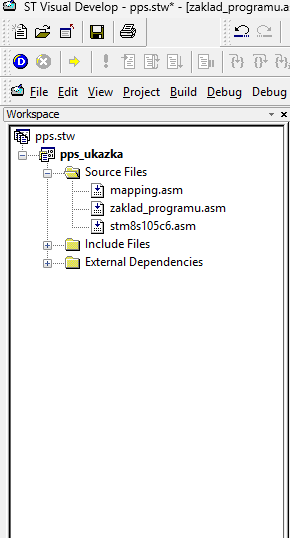
\includegraphics[width=1.00\textwidth]{fig/sim_prj.png}
			\end{center}
		\end{minipage}
		\begin{minipage}[t][\textheight][t]{0.75\textwidth}
		
		\small
		\begin{itemize}
			\item Soubory v projektu budou použity při překladu.
			
			\begin{itemize}
				\item \textbf{mapping.asm} - definice segmentů, v podstatě rozsahy adres pro paměťové celky.
					\begin{center}
						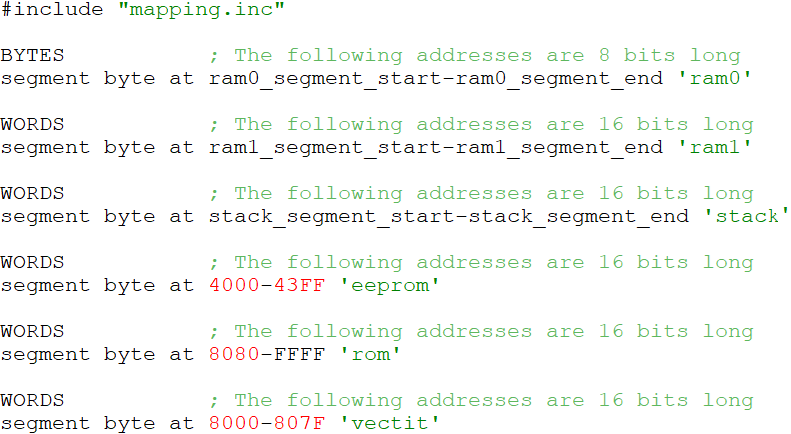
\includegraphics[width=0.70\textwidth]{fig/sim_mapping.png}
					\end{center}
				\item \textbf{stm8s105c6.asm} - pojmenování speciálních adres, tj. například registry \textbf{PA\_ODR}, \textbf{PA\_DDR} atd.
				\item \textbf{zaklad\_programu.asm} - náš zdrojový kód.
			\end{itemize}
			
		\end{itemize}
		
		\end{minipage}

	\end{frame}
	
% =====================================================================================================================
	\begin{frame}
    \frametitle{Program - vrchní část bez definic segmentů}
		
		\footnotesize
		\begin{center}
			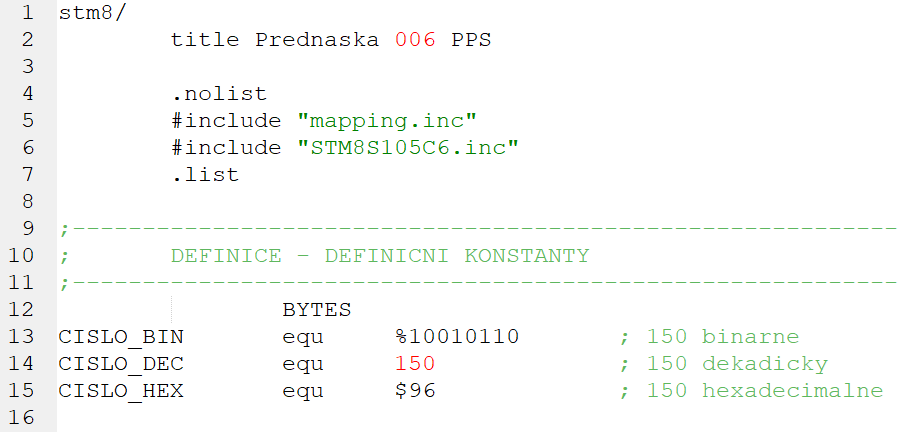
\includegraphics[width=0.85\textwidth]{fig/sim_prog_header.png}
		\end{center}
		
		\begin{enumerate}
			\item Vložení obsahu souborů \textbf{mapping.inc} a \textbf{STM8S105C6.inc} do našeho kódu.
			\item Vytvoření pojmenovaných konstant pomocí direktivy \textbf{\textcolor{blue}{EQU}}:
			
			\begin{itemize}
				\item všechny konstanty mají stejnou hodnotu \textbf{150},
				\item liší se číselnou soustavou ve které jsou zapsány.
			\end{itemize}
		\end{enumerate}

	\end{frame}
	
% =====================================================================================================================
	\begin{frame}
    \frametitle{Program - segmenty paměti dat a programu}
		
		\footnotesize
		\begin{center}
			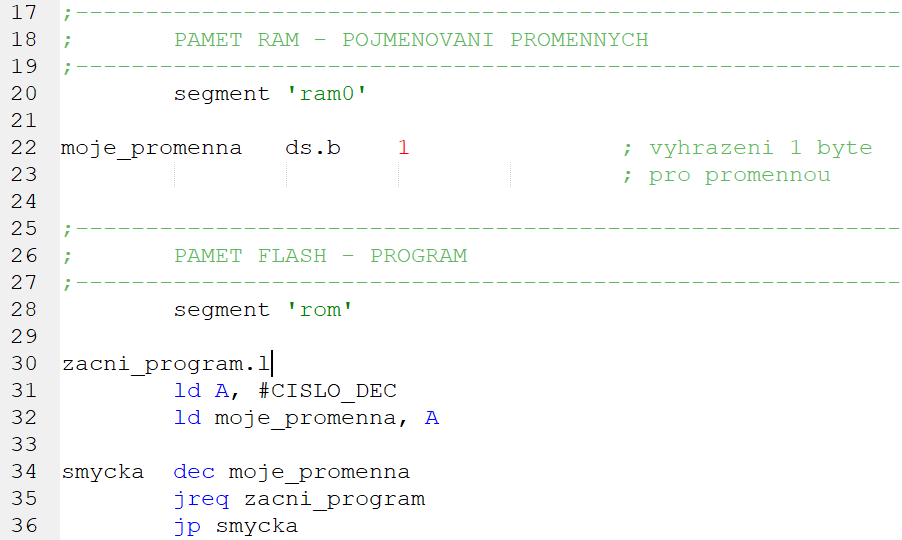
\includegraphics[width=0.85\textwidth]{fig/sim_prog_ram_rom.png}
		\end{center}
		
		\begin{enumerate}
			\item V segmentu RAM0 vyhrazujeme 1 byte pro proměnnou direktivou \textbf{\textcolor{blue}{ds.b}}.
			\item V segmentu ROM píšeme program pomocí instrukcí.
		\end{enumerate}

	\end{frame}
	
% =====================================================================================================================
	\begin{frame}
    \frametitle{Program - segment vektorů přerušení}
		
		\footnotesize
		\begin{center}
			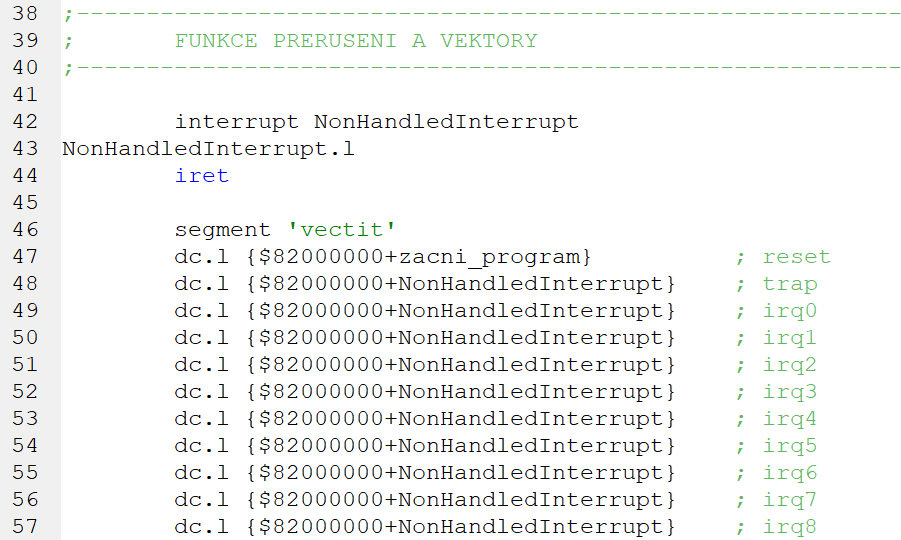
\includegraphics[width=0.85\textwidth]{fig/sim_prog_vectit.png}
		\end{center}
		
		\begin{enumerate}
			\item V segmentu VECTIT se procesor dozví první adresu skoku po resetu.
		\end{enumerate}

	\end{frame}